\section{Analysis and Design} \label{sec:AnalysisAndDesign}

As described by Bennett et al (\citeyear[][p.~348]{bennett2010object}), ``in
projects that follow an iterative life cycle, design is not such a clear-cut
stage, but rather an activity that will be carried out on the evolving model of
the system''. Seeing that the development method being followed in this project
is based on what should be an iterative approach, it was decided that the
analysis and design of it would be done concurrently.

The system will be designed in a layered architecture, and will consist of
three layers: \emph{presentation}, \emph{business Logic} and {persistence}. The
presentation layer will take care of the vast majority of the interactions
between the user and the system, and will depend only on the Business Logic
layer below it. The business logic will contain the model of the concepts which
will attempt to implement a solution to the problems outlined in the
requirements, and will depend only on the persistence layer below it. Lastly,
the persistence layer will ensure that the data is not lost when the
application is stopped (\cite[][p.~32-33]{bauer2016hibernate}). This approach
is also reminiscent of what has been described by Holmes
(\citeyear[][p.~3]{holmes2016mean}) as full stack development for an
application using a Model-View-Controller (MVC) architectural pattern, with one
of the differences being that the latter provides more details on how and when
the \emph{view} should be updated.

Regarding the modelling of the domain, Fowler
(\citeyear[][Section~1.3]{fowler1997analysis}) defines a pattern as ``an idea
that has been useful in one context and will probably be useful in others''.
So, analysis patterns will be used ``when trying to understand the problem''
domain (\cite[][Section~1.1]{fowler1997analysis}) in order to test this
concept, and as an attempt to make use of the experience already acquired in
the domain (or domains) in question. As emphasised by Bennett et al.
(\citeyear[][p.~252]{bennett2010object}), ``a pattern is useful when it
captures the essence of a problem and a possible solution, without being too
prescriptive''. So it may be the case that some of the patterns will be
modified where necessary to optimally solve a problem.

Essentially, an analysis pattern consists of a structure of classes and
associations which occurs often in many modelling situations related to
specific domains (\cite[][p.~254]{bennett2010object}).


Most of the aesthetic designs of the presentation layer happened in chapter
\ref{sec:Requirements.FunctionalRequirements}, so this one will focus on the
analysis and design of the business logic and persistence ones.

\subsection{Business Logic} \label{sec:AnalysisAndDesign.BusinessLogic}
Seeing that this is a system dealing with finance, it would make sense to treat
the categories as if they were treated as \emph{accounts}. So, in order to
make sure to imbue this system with knowledge acquired by more experienced
programmers, analysis and design patterns will be employed.

It is also useful at this point to make a distinction between the types of
classes used to model the domain between three possible kinds: the first are
the classes which model the interaction between the system and its actors --
these are called \emph{boundary classes}; the second kind are those classes
which model information and/or behaviour or some concept or phenomenon -- these
will be called \emph{entity classes}; and lastly, there are those classes which
model transactions, coordination, control and sequencing of other objects --
which are known as \emph{control classes} (Jacobson et al., 1999,
\cite[cited][pp.~198-201]{bennett2010object}).
%

The first analysis patterns which seem appropriate are a modified version of
the \emph{Account} pattern, used to create the \texttt{Category} entity class,
and the \emph{Quantity} pattern for the \texttt{Amount} entity class
(\cite[][Sections~6.1~\&~3.1]{fowler1997analysis}):
\begin{figure}[ht!]
  \begin{center}
    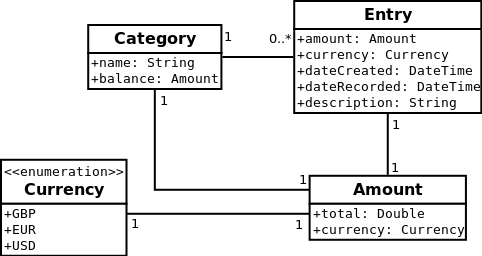
\includegraphics[width=10cm]{./contents/img/Class_Diagram_-_Categories_and_Amount.png}
  \end{center}
  \caption{}
  \label{fig:ClassDiagram.CategoriesAndAmount}
\end{figure}
\FloatBarrier

As implied by the diagram above, the \texttt{Category} class will be associated
with instances of the \texttt{Entry} class. This is done so that the only way to
change the total of a category is by adding positive or negative entries to it
-- for example, to indicate a credit to a category, a negative entry can be
added to it. One of the modifications to the original Account pattern consists
of the fact that, whereas in the original pattern an instance of
\texttt{Account} would keep track of the balance, there is no need to keep
track of the current balance in each \texttt{Category} -- the purpose of the
system is to allow the user to view a summary of income/expenditure by period,
so this will have to be calculated each time.

Another design choice which can be observed in Figure
\ref{fig:ClassDiagram.CategoriesAndAmount} is that the \texttt{Amount} class
also possesses an attribute for currency. This has been designed so as to allow
for the possibility of extending the system to keep track of transactions in
multiple currencies, although this was not a specific requirements. Initially,
there will only be a single default currency (GBP), so this will be hardcoded.
But the class should be implemented in a way which also allows for different
currencies to be loaded from another layer, such as the database, or an
external API.

The next step is to provide a way for these entries to be added to categories.
For this to happen, there needs to be a constraint to ensure that double entry
happens every time a change needs to be made to a category. One of the ways to
achieve this is to apply the \emph{Transaction} pattern
(\cite[][Section~6.2]{fowler1997analysis}):
\begin{figure}[ht!]
  \begin{center}
    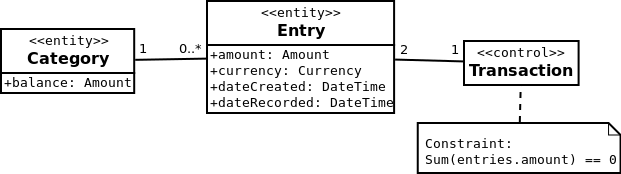
\includegraphics[width=9cm]{./contents/img/Class_Diagram_-_Transaction.png}
  \end{center}
  \caption{}
  \label{fig:ClassDiagram.Transaction}
\end{figure}
\FloatBarrier

After having determined some of the analysis patterns which shall be employed,
it makes sense to dive into a more specific analysis of the use cases described
in Chapter \ref{sec:Requirements}. At this point the objective will be to start
modelling classes and interactions based on concepts or things found in the
problem domain. This will be done in the following subsections.

\subsubsection{Create Manual Entry} \label{sec:AnalysisAndDesign.BusinessLogic.ManualEntry}

%TODO: check if this diagram still makes sense after implementation
The \emph{Create Manual Entry} use case, which allows a
user to input financial transactions individually using a specific interface,
can be modelled as follows (Figure \ref{fig:CommDiagram.CreateManualEntry}):
\begin{figure}[ht!]
  \begin{center}
    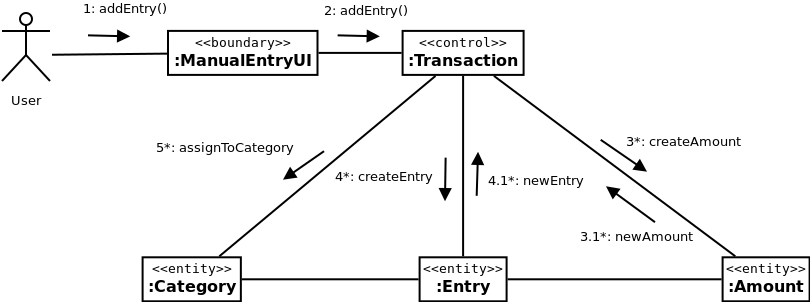
\includegraphics[width=12cm]{./contents/img/Comm_Diagram_-_Manual_Entry.png}
  \end{center}
  \caption{Communication Diagram for the \emph{Create Manual Entry} use case}
  \label{fig:CommDiagram.CreateManualEntry}
\end{figure}
\FloatBarrier

As the diagram above indicates, the \texttt{Transaction} class is responsible for
the creation of new instances of \texttt{Entry} and \texttt{Amount}, which then get
assigned to the \texttt{Category} instances chosen, or created, by the user.
Once the user starts typing, the \texttt{CategorySuggester} is triggered to
suggest categories. The actual implementation of how this suggestions happen
may vary, but initially it should at least be based on what the user types in
the search box. If the user chooses to create a new category instead, then they
will be taken to the appropriate interface to allow them to do so. Once the
user is satisfied and chooses to submit, the system will start to input the
transactions in the appropriate category or categories.

Although \texttt{Transaction} was originally thought of as a \emph{control
class}, it was later decided that it would be beneficial to save the
transaction information, so it was made into an \emph{entity class} instead.
It is also worth noting that, although implicit in the diagram and the
wireframe on Figure \ref{fig:Wireframe.CreateManualEntry}, it is estimated that
the user will start the interface, enter the transaction's details, and then
start the process to find a category. Seeing that there will be a search
suggestion at this point, it felt it was appropriate to have the diagram on
Figure \ref{fig:CommDiagram.CreateManualEntry} have its first message sent at
this stage.

It is also important to emphasise the fact that \texttt{CategorySuggester} is
only an interface at this point, and that the suggester in the diagram will be
any object which implements this interface. This is to allow more flexibility
in the implementation of the classes responsible for suggesting categories to
the user.

\subsubsection{Upload Statement} \label{sec:AnalysisAndDesign.BusinessLogic.UploadStatement}

The user should be able to upload their bank statements, provided that they are
in a suitable format. The specifics of the format will be described in the
implementation phase, together with more information on how to encapsulate as
much as possible the complexities related to the formatting of this
information.  For the analysis and design phases, the emphasis will be on
modelling the objects and their interactions. The diagram (Figure
\ref{fig:CommDiagram.CreateManualEntry}) below illustrates this process:
\begin{figure}[ht!]
  \begin{center}
    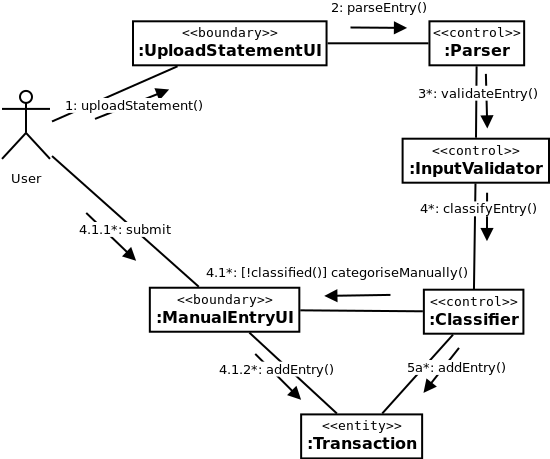
\includegraphics[width=14cm]{./contents/img/Comm_Diagram_-_Upload_Statement.png}
  \end{center}
  \caption{Communication Diagram for the \emph{Upload Statement} use case}
  \label{fig:CommDiagram.CreateManualEntry}
\end{figure}
\FloatBarrier

As can be seen in the diagram above, the process is spread among many classes.
After the user uploads the statement, the loaded raw input will be sent to a
\texttt{Parser} which will separate it according to the columns into the
appropriate fields and line items. Then, what is now a collection of statement
line items will be passed on to an \texttt{InputValidator} to make sure the user
input is valid. Lastly, the resulting validated entries will be sent down to a
\texttt{Classifier}, which will signal the relevant \texttt{Transaction}
instance(s) to add the entries to their relevant \texttt{Category} instances --
this last part has already been illustrated in Figure
\ref{fig:CommDiagram.CreateManualEntry}. 

When the \texttt{Classifier} cannot match a line item against any of the existing
categories, it will pass the line in question to the \texttt{ManualEntryUI},
which, apart from having all transaction details already populated, will rely
on the process described at subsection \ref{sec:AnalysisAndDesign.BusinessLogic.ManualEntry}
to properly categorise the item and then forward it to \texttt{Transaction} to
create the categories.

\subsubsection{Visualise Categorised Summary} \label{sec:AnalysisAndDesign.BusinessLogic.ViewSummary}
As mentioned before, this feature will allow the user to view a summary of
their income and expenditure by category.  The user will enter the period which
they want to examine, and the system will retrieve the categories which have
entries with those dates.  The system should then sort the categories by income
or expenditure and by total, and then display it to the user. Optionally, the
user can filter the output further by choosing a single category.

Below (Figure \ref{fig:CommDiagram.VisualiseCategorisedSummary}) is a
communication diagram to illustrate this interaction: 
\begin{figure}[ht!]
  \begin{center}
    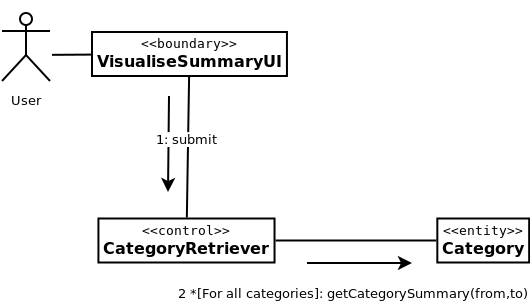
\includegraphics[width=12cm]{./contents/img/Comm_Diagram_-_Visualise_Categorised_Summary.png}
  \end{center}
  \caption{communication diagram for \emph{Visualise Categorised Summary} use case}
  \label{fig:CommDiagram.VisualiseCategorisedSummary}
\end{figure}
\FloatBarrier



\subsubsection{Calculate Budget} \label{sec:AnalysisAndDesign.BusinessLogic.CalculateBudget}
This feature will allow the user to request the system to calculate a budget
for them over a period of time. What the system will do then is retrieve all
categories over the last 12 months, then calculate their means and take them as
ratio of the income over the same last period. Then, it will take the first few
which make up more than 80\% of the total, and add all the others which make up
the remainder and add them up as `other' or something similar. It will then
show these totals to the user, in a similar way as it shows the categorised
summary. The communication diagram below (Figure
\ref{fig:CommDiagram.CalculateBudget}) illustrates the steps taken by the
application layer.

\begin{figure}[ht!]
  \begin{center}
    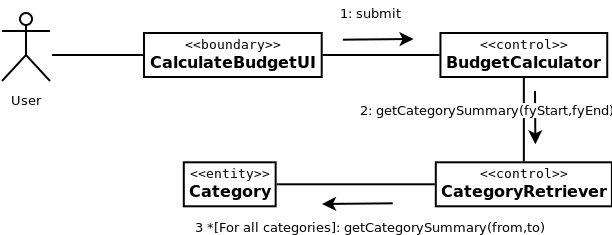
\includegraphics[width=14cm]{./contents/img/Comm_Diagram_-_Calculate_Budget.png}
  \end{center}
  \caption{communication diagram for \emph{Calculate Budget}}
  \label{fig:CommDiagram.CalculateBudget}
\end{figure}
\FloatBarrier


\subsubsection{Final Class Diagram} \label{sec:AnalysisAndDesign.BusinessLogic.FinalClassDiagram}
The class diagram on Figure \ref{fig:ClassDiagram.AllClasses} is the result of
joining the more relevant entities listed so far:
\begin{figure}[ht!]
  \begin{center}
    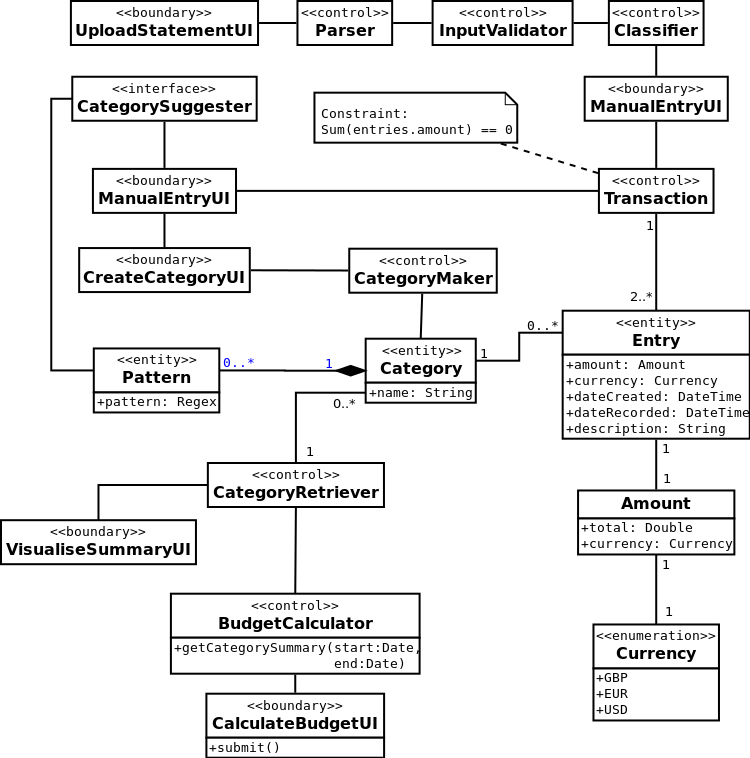
\includegraphics[width=15cm]{./contents/img/Class_Diagram_-_All_Classes.png}
  \end{center}
  \caption{Class diagram of the most relevant classes of the Business Logic Layer}
  \label{fig:ClassDiagram.AllClasses}
\end{figure}
\FloatBarrier

Manual entries and uploaded statements will inevitably always go against a Bank
category. For this reason, there does not seem to be any harm in hard-coding
the \texttt{Bank} category. In this case, since most transactions are going to
affect it, it was decided that no patterns should be assigned to it. Due to
this, it was decided to allow multiplicity of \texttt{0..*} to the association
between \texttt{Pattern} and \texttt{Category}. This relationship has also been
made into a composition, since patterns should not exist without categories on
the system, but a category can exist without a pattern.


\subsection{The Persistence Layer} \label{sec:AnalysisAndDesign.PersistenceLayer}
This is the layer which communicates directly with the database. It tries to
encapsulate as much as possible the details of how it accesses the outside
world by only exposing one singleton object, the \texttt{PersistenceMediator}.
This is the object responsible for manipulating the database, with the help of
other encapsulated package members. It uses a \emph{Java Properties} file to
choose which database engine to use (at the moment only \emph{MySql} and
\emph{H2} are available), but 

\subsection{Database Diagram} \label{sec:AnalysisAndDesign.PersistenceLayer}
The UML diagram below shows the design of the database schema for the
application:
\begin{figure}[ht!]
  \begin{center}
    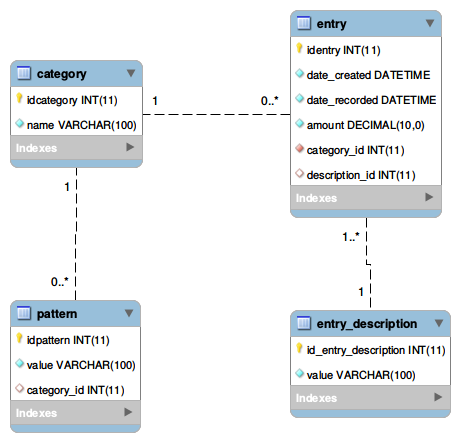
\includegraphics[width=14cm]{./contents/img/Database_Diagram.png}
  \end{center}
  \caption{UML Diagram of database schema}
  \label{fig:ClassDiagram.AllClasses}
\end{figure}
\FloatBarrier

As the diagram indicates, the entities and relationships of the database are
very similar to those of the business logic layer, except that it was felt
that, since due to double-entry the \texttt{Entry} instances will occur
multiple time, the description should be given a table of its own in order to
contribute to optimising storage space used.

One of the main reasons for choosing to model the application logic first, and
then model the database, was that it would be more likely to ensure that the
model (data structure) would reflect the needs of the application more
accurately, as stated by Holmes (\citeyear[][p.~141]{holmes2018mean}). Also
according to Holmes, the risk of having the model of the data adversely affect
how the application will work and behave can be higher if the application
design starts with the data model.
